\section{应用}

本章将介绍联邦学习技术在一些应用场景中的应用,包括移动设备上的应用、车辆驾驶领域的应用等。

\subsection{联邦学习在移动设备上的应用}

% 介绍移动设备上语音助手的现状和存在的问题
移动设备上的语音助手,如Siri、Google Assistant等,已经成为人们日常生活中的重要组成部分。这些语音助手可以帮助用户完成一些简单的任务,如查询天气、播放音乐等。然而,由于模型需要处理大量的用户数据,用户的隐私安全问题成为了一个严重的问题。传统的移动模型的训练需要大量用户数据,这一过程通常会将用户的数据上传到云端进行处理,这样会导致用户的隐私数据泄露的风险。

% 介绍联邦学习在移动设备上的应用
为了解决这个问题,研究者提出了使用联邦学习技术部署在移动设备上方法\cite{kang2020reliable,lim2020federated}。这种方法的基本思想是在移动设备上训练一个本地模型,然后将本地模型上传到服务器,服务器对本地模型进行聚合,得到全局模型。这样可以避免用户的隐私数据泄露。联邦学习在移动设备上的应用可以提高用户的隐私安全性,同时提高语音助手的性能。

如图\ref{fig:mobile}所示,传统的模型学习方法需要将用户的数据上传到云端进行处理,这样会导致用户的隐私数据泄露的风险。而联邦学习技术可以在移动设备上进行模型训练,避免了用户的隐私数据泄露的风险。联邦学习在移动设备上的应用可以分为以下几个步骤:

\begin{figure}[htbp]
    \centering
    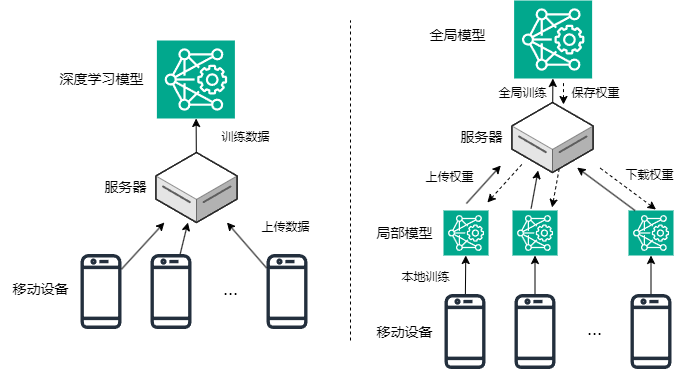
\includegraphics[width=\textwidth]{images/mobile.png}
    \caption{联邦学习在移动设备上的应用}
    \label{fig:mobile}
\end{figure}

\begin{enumerate}
    \item 移动设备上的本地模型训练:移动设备上的本地模型使用用户的语音数据进行训练。
    \item 本地模型上传到服务器:本地模型将训练好的模型上传到服务器。
    \item 服务器对本地模型进行聚合:服务器对本地模型进行聚合,得到全局模型。
    \item 全局模型下发到移动设备:服务器将全局模型下发到移动设备,移动设备使用全局模型进行推理。
    \item 移动设备上的本地模型更新:移动设备上的本地模型使用全局模型进行推理,然后将推理结果上传到服务器,服务器使用这些结果更新全局模型。
    \item 重复步骤2-5,直到模型收敛。
\end{enumerate}

\subsection{联邦学习在车辆驾驶领域的应用}

% 介绍车辆驾驶的现状和存在的问题
车辆驾驶是一个复杂的任务,需要驾驶员不断地观察周围的环境,做出相应的决策。传统的车辆驾驶系统通常使用固定的规则来控制车辆的行驶,这样会导致车辆的行驶效果不佳。为了提高车辆的行驶效果,传统的想法是收集大量的车辆数据,然后使用这些数据训练一个模型,来控制车辆的行驶。然而,由于车辆驾驶环境的复杂性和实时性,传统的方法很难满足实际的需求。

% 介绍联邦学习在车辆驾驶领域的应用
为了解决这个问题,研究者提出了使用联邦学习技术在车辆驾驶领域的应用\cite{posner2021federated,du2020federated}。联邦学习技术可以在车辆之间共享模型,同时为每辆车提供个性化的模型。这样可以提高车辆的行驶效果,同时减少车辆之间的通信开销。

如图\ref{fig:car}所示,传统的模型学习方法需要将车辆的数据上传到云端进行处理,这样会导致通信开销较大,且网络传输延迟时间长。而联邦学习技术可以为每辆车提供个性化的模型,同时直接与本地局部模型通信,大量减少延迟,满足行驶环境下的实时性需求。联邦学习在车辆驾驶领域的应用可以分为以下几个步骤:

\begin{figure}[htbp]
    \centering
    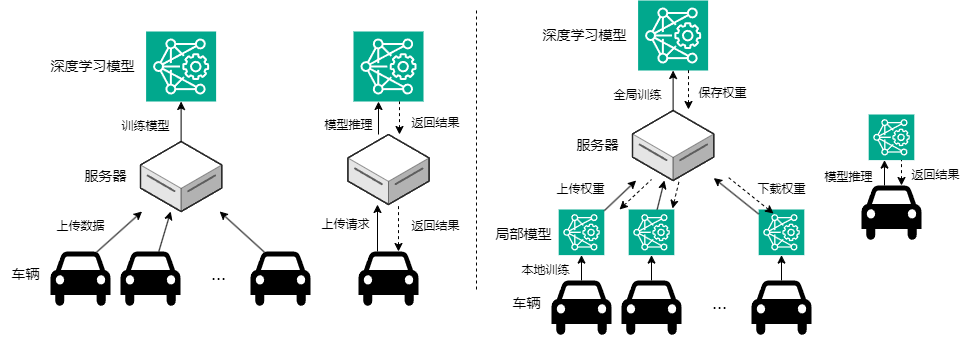
\includegraphics[width=\textwidth]{images/car.png}
    \caption{联邦学习在车辆驾驶领域的应用}
    \label{fig:car}
\end{figure}

\begin{enumerate}
    \item 车辆上的本地模型训练:每辆车使用自己的数据训练本地模型。
    \item 本地模型上传到服务器:每辆车将训练好的模型上传到服务器。
    \item 服务器对本地模型进行聚合:服务器对本地模型进行聚合,得到全局模型。
    \item 全局模型下发到车辆:服务器将全局模型下发到车辆,车辆使用全局模型进行推理。
    \item 车辆上的本地模型更新:车辆使用全局模型进行推理,然后将推理结果上传到服务器,服务器使用这些结果更新全局模型。
    \item 重复步骤2-5,直到模型收敛。
    \item 车辆上的本地模型推理:车辆使用本地局部模型进行推理,快速得到控制车辆行驶的决策。
\end{enumerate}

\subsection{联邦学习在其他领域的应用}

除了在移动设备和车辆驾驶领域的应用,联邦学习技术还可以在其他领域进行应用。例如,在金融领域,联邦学习技术可以用于风险评估、信用评分等任务。考虑到各个金融机构之间的数据隐私性,联邦学习技术可以在不泄露用户隐私的情况下,共享模型,提高金融机构的风险评估能力\cite{saputra2020federated}。此外,在医疗领域,联邦学习技术可以用于医疗影像诊断、疾病预测等任务。医疗数据的隐私性是医疗领域的一个重要问题,联邦学习技术可以在不泄露患者隐私的情况下,共享模型,提高医疗诊断的准确性\cite{sheller2020federated}。